% 保留原始面板、实拍、示例与全部连线；仅以 TikZ 覆盖说明标签。
\begin{tikzpicture}
\node[anchor=south west,inner sep=0] (im) at (0,0) {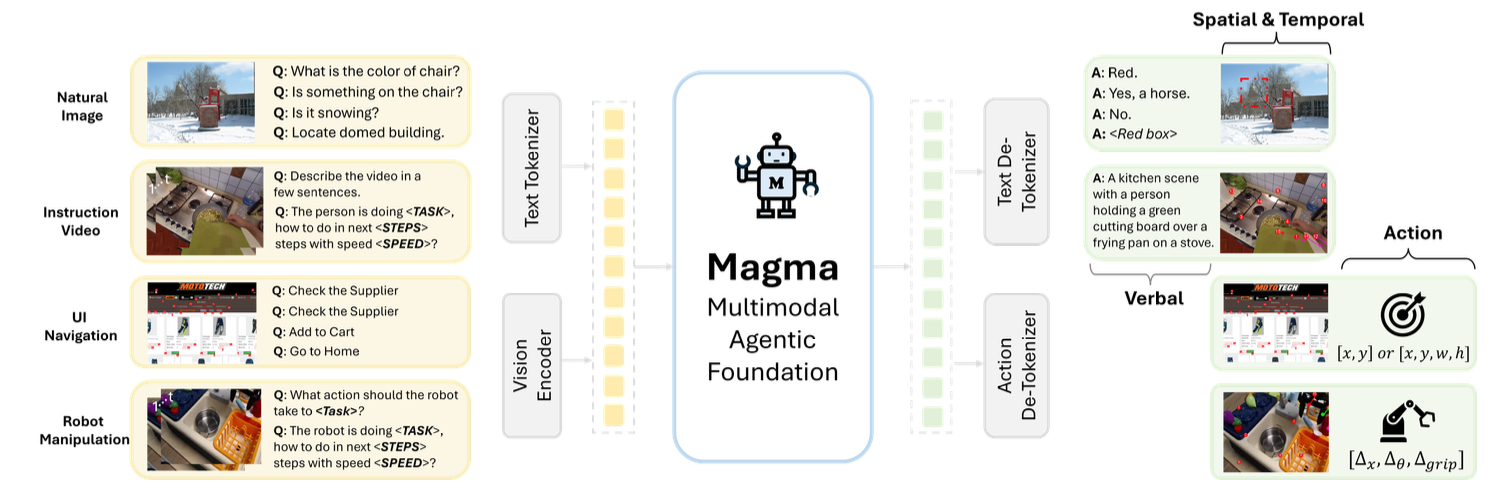
\includegraphics[width=\linewidth]{figures/magma.png}};
\begin{scope}[x={(im.south east)},y={(im.north west)}]
\fill[white] (0.029570,0.743902) rectangle (0.081989,0.821138);
\node[align=center,inner sep=0pt,font=\fontsize{8}{9}\selectfont,text width=0.052419\linewidth,rotate=0] at (0.055780,0.782520) {自然图像};
\fill[white] (0.025538,0.506098) rectangle (0.081989,0.587398);
\node[align=center,inner sep=0pt,font=\fontsize{8}{9}\selectfont,text width=0.056452\linewidth,rotate=0] at (0.053763,0.546748) {指令视频};
\fill[white] (0.026882,0.296748) rectangle (0.081317,0.376016);
\node[align=center,inner sep=0pt,font=\fontsize{8}{9}\selectfont,text width=0.054435\linewidth,rotate=0] at (0.054099,0.336382) {界面导航};
\fill[white] (0.023522,0.048780) rectangle (0.087366,0.191057);
\node[align=center,inner sep=0pt,font=\fontsize{7.5}{8.5}\selectfont,text width=0.063844\linewidth,rotate=0] at (0.055444,0.119919) {机器人\\操作};
\fill[white] (0.338710,0.510163) rectangle (0.372312,0.788618);
\node[align=center,inner sep=0pt,font=\fontsize{7.5}{8.5}\selectfont,text width=0.033602\linewidth,rotate=0] at (0.355511,0.649390) {文本\\词元化器};
\fill[white] (0.338710,0.123984) rectangle (0.373656,0.392276);
\node[align=center,inner sep=0pt,font=\fontsize{7.5}{8.5}\selectfont,text width=0.034946\linewidth,rotate=0] at (0.356183,0.258130) {视觉\\编码器};
\fill[white] (0.460349,0.193089) rectangle (0.580645,0.410569);
\node[align=center,inner sep=0pt,font=\fontsize{9}{10}\selectfont,text width=0.120296\linewidth,rotate=0] at (0.520497,0.301829) {多模态\\智能体\\基础模型};
\fill[white] (0.661962,0.512195) rectangle (0.702285,0.792683);
\node[align=center,inner sep=0pt,font=\fontsize{7.5}{8.5}\selectfont,text width=0.040323\linewidth,rotate=0] at (0.682124,0.652439) {文本反\\词元化器};
\fill[white] (0.663306,0.121951) rectangle (0.701613,0.384146);
\node[align=center,inner sep=0pt,font=\fontsize{7.5}{8.5}\selectfont,text width=0.038306\linewidth,rotate=0] at (0.682460,0.253049) {动作反\\词元化器};
\fill[white] (0.797043,0.932927) rectangle (0.927419,0.985772);
\node[align=center,inner sep=0pt,font=\fontsize{8.5}{9.5}\selectfont,text width=0.130376\linewidth,rotate=0] at (0.862231,0.959350) {空间与时间};
\fill[white] (0.749328,0.367886) rectangle (0.805108,0.416667);
\node[align=center,inner sep=0pt,font=\fontsize{8.5}{9.5}\selectfont,text width=0.055780\linewidth,rotate=0] at (0.777218,0.392276) {语言};
\fill[white] (0.927419,0.502033) rectangle (0.979839,0.550813);
\node[align=center,inner sep=0pt,font=\fontsize{8.5}{9.5}\selectfont,text width=0.052419\linewidth,rotate=0] at (0.953629,0.526423) {动作};
% 完整中文化问答示例；数值词元、占位符、照片与连线保持原样。
\fill[yellow!9] (0.181452,0.709350) rectangle (0.312500,0.873984);
\node[anchor=north west,align=left,inner sep=0pt,font=\fontsize{4.8}{5.4}\selectfont,text width=0.128360\linewidth] at (0.182796,0.869919) {问：椅子是什么颜色？\\问：椅子上有东西吗？\\问：在下雪吗？\\问：定位圆顶建筑。};
\fill[yellow!9] (0.181452,0.483740) rectangle (0.312500,0.652439);
\node[anchor=north west,align=left,inner sep=0pt,font=\fontsize{5.0}{5.8}\selectfont,text width=0.128360\linewidth] at (0.182796,0.648374) {问：用几句话描述视频。\\问：此人正做\texttt{<TASK>}；\\接下来如何以\texttt{<SPEED>}\\速度完成\texttt{<STEPS>}步？};
\fill[yellow!9] (0.181452,0.270325) rectangle (0.312500,0.426829);
\node[anchor=north west,align=left,inner sep=0pt,font=\fontsize{5.0}{5.4}\selectfont,text width=0.128360\linewidth] at (0.182796,0.422764) {问：查看供应商\\问：查看供应商\\问：加入购物车\\问：回到首页};
\fill[yellow!9] (0.181452,0.034553) rectangle (0.312500,0.223577);
\node[anchor=north west,align=left,inner sep=0pt,font=\fontsize{4.6}{5.0}\selectfont,text width=0.128360\linewidth] at (0.182796,0.219512) {问：机器人应如何\\完成\texttt{<Task>}？\\问：机器人正做\texttt{<TASK>}；\\接下来如何以\texttt{<SPEED>}\\速度完成\texttt{<STEPS>}步？};
\fill[green!6] (0.731855,0.709350) rectangle (0.817204,0.873984);
\node[anchor=north west,align=left,inner sep=0pt,font=\fontsize{4.6}{5.1}\selectfont,text width=0.082661\linewidth] at (0.733199,0.869919) {答：红色。\\答：是，一匹马\\答：没有。\\答：\texttt{<Red box>}};
\fill[green!6] (0.731855,0.483740) rectangle (0.817876,0.654472);
\node[anchor=north west,align=left,inner sep=0pt,font=\fontsize{5.0}{5.5}\selectfont,text width=0.083333\linewidth] at (0.733199,0.650407) {答：厨房中，一人手持绿色切菜板，悬在灶台上的煎锅上方。};
\end{scope}
\end{tikzpicture}
